\section{Configuration Management}  \label{configmgmt}
Da eine der Anforderungen an unsere Produktentwicklung die einfache Erweiterbarkeit war, mussten wir einen Weg finden, die Einstellungen, die sich von Kunde zu Kunde unterscheiden, einfach zu ändern.  \\
Die Lösung, die es uns ermöglichen würde, dies zu erreichen, wäre die zentrale Speicherung der Konfigurationsdateien, so dass diese leicht gefunden und bearbeitet werden kann, ohne den Code selbst bearbeiten zu müssen. Wir haben zwei Standardstrategien gefunden, um dieses Ziel zu erreichen. Die erste besteht darin, das eingebaute Key-Value store von Consul zu nutzen (welcher aber immer noch als Discovery Service genutzt wird). Die zweite Strategie wäre, das Spring Cloud Config-Paket zu verwenden und einen separaten Microservice aufzubauen, der für die Verwaltung der Konfigurationsdateien bestimmter Services zuständig ist. 
\namedsubsection{Consul}{J}
Consul ist eine Software, welche von der HashiCorp Group entwickelt wird. Sie wird hauptsächlich angewendet um im Cloud Bereich verschiedene (Micro-)Services zu vernetzen und diese zentral über ein Register kommunizieren zu lassen. Consul verfügt sowohl über ein Command Line Interface, als auch über ein User Interface, welches standardisiert mitgeliefert wird und eine einfache Handhabung über den Browser auf Port 8500 ermöglicht.

Einige für uns relevanten Kernfunktionalitäten von Consul sind:

\begin{itemize}
  \item \textbf{Discovery Service:}
    Einzelnen (Micro-)Services können sich bei Consul registrieren und nachfolgend auf andere bereits registrierte Services zugreifen (vgl Abb. \ref{fig:service_registration_consul}). Diese Registrierung findet über die von Consul bereitgestellte Schnittstelle statt. Innerhalb von Consul lassen sich auch über die sogenannten Intentions festlegen, welche Services mit welchen anderen Services kommunizieren dürfen.
    \item \textbf{Health Checking:}
    Consul überprüft mittels dem Heartbeat Protokol für jeden registrierten Service ob dieser noch läuft oder ob dieser gestoppt hat. Der Standard Heartbeat erfolgt alle 10 Sekunden.
    \item \textbf{Key Value Store:}
    Innerhalb von Consul lassen sich Key-Value Paare abspeichern, welche dann allen Services mittels einer einfachen HTTP Schnittstelle zur Verfügung stehen. Hierüber lassen sich beispielsweise Konfigurationen, wie z.B lokale Datenbankadressen, Passwörter etc. sehr gut einheitlich für alle Services anpassen. Auf diese Art lassen sich sowohl einfache Werte, wie auch komplette Dateien, wie z.B eine YAML-Konfigurations Datei zentral, für alle Services verfügbar, abspeichern.
    \item \textbf{Secure Service Communication:}
    Zwischen den einzelnen Servicen kann TLS Kommunikation verwendet werden.

\end{itemize}

\begin{figure}[!h]
\centering
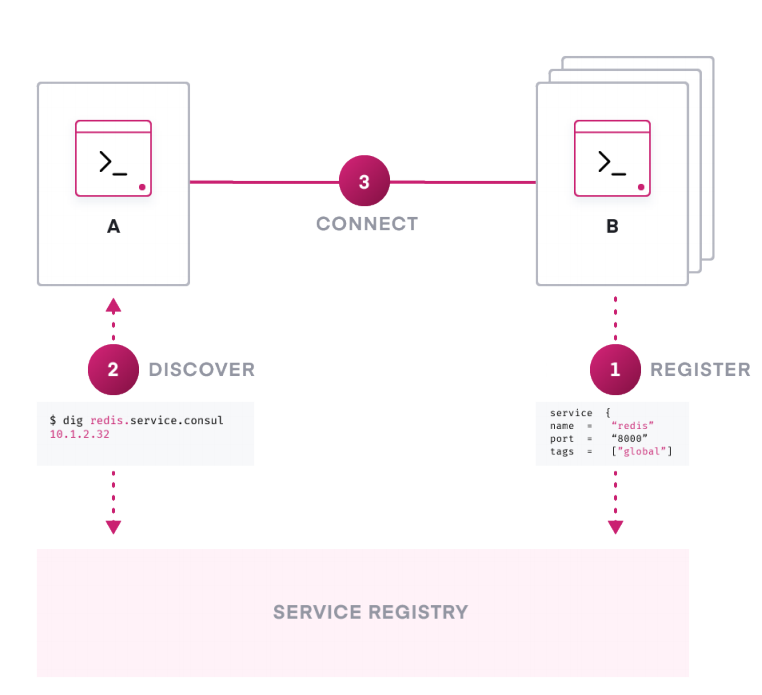
\includegraphics[width=10cm]{images/07_Consul/Consul_register.png}
\caption{Ablauf einer Service Registrierung bei Consul}
\cite{consul}
\label{fig:service_registration_consul}
\end{figure}


Nach der Installation von Consul kann dessen graphische Oberfläche über den Port 8500 angesprochen werden (localhost:8500). 

Um von anderen Servicen angesprochen werden zu können registriert sich ein einzelner Service bei seiner Initialisierung bei Consul (vgl Abb. \ref{fig:service_registration_consul}). Im Folgenden können andere Services die Addressen der bereits initialisierten Services anfragen und, falls Sie hierfür die Berechtigung besitzen direkt mit Ihnen kommunizieren. Die Kommunikation findet ausdrücklich nicht über Consul selbst, sonder zwischen den einzelnen Servicen statt. Des Weiteren überprüft Consul mittels seines Heartbeats, also einem periodischen Ping an alle Services ob ein Dienst ausgefallen ist. Für diesen Fall lassen sich verschiedene Eskalationsszenarien integrieren.

\namedsubsection{Cloud Config}{M}
%Wie funktioniert?
%Warum Overhead?
Spring Cloud Config bietet serverseitige und clientseitige Unterstützung für die externalisierte Konfiguration in einem verteilten System. Bei dieser Lösung wird mit Hilfe der im Cloud-Paket verfügbaren Annotation $@EnableConfigServer$ ein dedizierter Server aufgebaut, auf den von der Ebene jedes einzelnen Dienstsystems aus zugegriffen werden kann und der als zentrale Stelle für die Verwaltung der Anwendungseigenschaften fungiert.\\ Die Standardimplementierung des Server-Speicher-Backends verwendet git, so dass es problemlos etikettierte Versionen von Konfigurationsumgebungen unterstützt und für eine breite Palette von Werkzeugen zur Verwaltung der Inhalte zugänglich ist. Natürlich muss der Config-Server wissen, wo die Dateien mit den Anwendungseigenschaften verfügbar sind. Aus diesem Grund sollte die Adresse eines Git-basierten Repositorys (wie Github oder Gitlab), in dem die Konfigurationsdateien gespeichert werden, in die eigenen Eigenschaften aufgenommen werden. Eine alternative Lösung besteht darin, das neue Git-Repository auf Ihrer Festplatte zu initialisieren und einen Pfad zu ihm anzugeben, wenn Sie Ihre Konfigurationen nicht in der Cloud speichern möchten. \\
Die Spring Cloud Config muss auch wissen, welcher Dienst welche Konfigurationseigenschaften zur Verfügung stellt. Dieses Problem wurde so gelöst, dass der Name der Konfigurationsdatei mit dem in den lokalen Eigenschaften angegebenen Dienstnamen übereinstimmen muss. Dies bedeutet, dass die in der Datei $test$-$service.properties$ enthaltenen Eigenschaften dem Dienst mit der Eigenschaft $spring.application.name=test$-$service$ zugeordnet werden. \\
Auf der anderen Seite müssen die Dienste auch wissen, wie sie sich mit dem Konfigurationsserver verbinden können. In einer Standardkonfiguration brauchen Sie nur die $org.springframework.cloud$:$spring$-$cloud$-$starter$-$config$ hinzuzufügen, die die Anwendung im Hintergrund automatisch so konfiguriert, dass sie mit einer zentralen Konfiguration beginnen kann.
\namedsubsection{Consul vs Cloud Config}{M}
Schließlich entschieden wir uns für das integrierte Key-Value Store des Consuls. Der Faktor, der den größten Einfluss auf unsere Entscheidung hatte, war die Komplexität der spezifischen Lösungen. Da das mit beiden Lösungen erzielte Endergebnis im Grunde genommen dasselbe ist, sind wir zu dem Schluss gekommen, dass es nicht notwendig ist, dem System eine zusätzliche Komponente hinzuzufügen, die eine zusätzliche Fehlerquelle darstellen könnte. Obwohl die Spring Cloud Config in Bezug auf die einfache Verwaltung bestimmter Dienste besser abschneidet, waren die Vorteile in unseren Augen nicht ausschlaggebend genug um den verbundenen Mehraufwand zu rechtfertigen. Vor allem, wenn man den Umfang unseres Systems betrachtet, das nur einige wenige Mikrodienste enthält. \\
Darüber hinaus bevorzugt Statistance die lokale Speicherung von Konfigurationsdateien, so dass der Vorteil der Möglichkeit, git-Repositorys zur Speicherung von Anwendungseigenschaften zu verwenden, nicht anwendbar ist. Die oben genannten Argumente haben uns davon überzeugt, dass Consul und sein Key-Value-Store für diesen speziellen Fall besser geeignet sind, da Consul eine zweite wichtige Rolle in unserem System hat, nämlich die Service-Discovery.